\documentclass[tikz,border=1pt]{standalone}
% Shared style of the Background schematics (bg_*.tex).  Colors follow figures/bar_patterns.py: each hue keeps one
% meaning across the paper (orange = required output / WISEConv, teal = tile skipping, violet = gather-scatter extra
% data, dotted gray = wasted computation, as in fig:gap).  Drawn at \columnwidth (241 pt), included unscaled.  Cell fills and
% the dark-navy rules come from the authors' original schematics (input C1E5F5, weights F2CFEE, required FBE3D6);
% the SM fill is a lighter step of their D9D9D9 so that it stays apart from the wasted gray.
\usepackage[T1]{fontenc}
\usepackage[tt=false,type1=true]{libertine}
\usepackage[libertine]{newtxmath}
\usepackage{tikz}
\usetikzlibrary{arrows.meta,calc,patterns.meta,positioning,fit,backgrounds,decorations.pathreplacing}

\definecolor{ink}{HTML}{222222}
\definecolor{muted}{HTML}{6B6B68}
\definecolor{rule}{HTML}{2A4552}
\definecolor{wiseconv}{HTML}{DD7428}
\definecolor{tileskip}{HTML}{26A08F}
\definecolor{gather}{HTML}{9877CC}
\definecolor{wasted}{HTML}{DDDDDD}
\definecolor{wastedink}{HTML}{9A9A9A}
\definecolor{infill}{HTML}{C1E5F5}
\definecolor{wfill}{HTML}{F2CFEE}
\definecolor{smfill}{HTML}{EAEAEA}
\definecolor{actfill}{HTML}{FBE3D6}
\colorlet{gsfill}{gather!45!white}

\tikzset{
  every picture/.style={line join=round, line cap=round, font=\fontsize{8}{9.6}\selectfont, color=ink},
  cell/.style={draw=rule, line width=0.35pt, minimum size=#1, inner sep=0pt, outer sep=0pt, anchor=north west},
  cell/.default=3.6mm,
  idx/.style={font=\fontsize{6.8}{7}\selectfont, text=ink!85},
  act/.style={fill=actfill},
  inp/.style={fill=infill},
  wgt/.style={fill=wfill},
  waste/.style={fill=wasted, postaction={pattern={Dots[distance=1.2pt, radius=0.22pt]}, pattern color=wastedink}},
  gs/.style={fill=gsfill},
  sm/.style={fill=smfill, rounded corners=2pt, draw=none},
  mem/.style={fill=white, draw=rule, line width=0.4pt, rounded corners=1.2pt},
  smlabel/.style={font=\fontsize{6.8}{7}\selectfont\scshape, text=muted, anchor=north west, inner sep=1.4pt},
  flow/.style={-{Stealth[length=3.2pt, width=2.6pt]}, line width=0.55pt, draw=ink},
  title/.style={font=\fontsize{8}{9}\selectfont, anchor=north, inner sep=1pt},
  op/.style={font=\fontsize{9.5}{10}\selectfont, text=ink},
}

% \grid{x}{y}{cols}{rows}{size}{style of cell i (macro taking the index)}{first index label or empty}
\newcommand{\cellat}[4]{% x, y (top-left), size, style
  \node[cell=#3, #4] at (#1, #2) {};}

\usepackage{pifont}
% fig:overview: WISEConv on the running example (active outputs 0, 5, 9, 12, 14).  (1) One construction pass compacts
% each 2x2 construction tile of M_out into a segment and appends it to the worklist W in arrival order; the same pass
% places the length n_W against the layer's thresholds and selects the tile configuration.  (2) Geometry-compatible
% operators reuse W; a stride-2 layer rebuilds it.  (3) A persistent grid consumes W in tiles of the selected size;
% each row reads its receptive field from the dense input in place and the reduction is the dense one.  Bottom: the
% per-frame CUDA graph: the host launches it once; construction enables one of the layer's candidate compute nodes.
\colorlet{selfill}{wiseconv!55!white}
\colorlet{altfill}{wiseconv!18!white}
\tikzset{
  box/.style={draw=rule!55, line width=0.5pt, rounded corners=2.5pt},
  boxtitle/.style={anchor=north west, font=\fontsize{8}{9}\selectfont\bfseries, inner sep=1.6pt},
  note/.style={font=\fontsize{6.8}{7.4}\selectfont, text=muted},
  node box/.style={draw=rule, line width=0.45pt, rounded corners=1.2pt, minimum height=5.4mm, inner sep=1.2pt,
                   font=\fontsize{6.8}{7.4}\selectfont, align=center},
}
\newcommand{\num}[1]{\ding{\numexpr191+#1\relax}}
\begin{document}
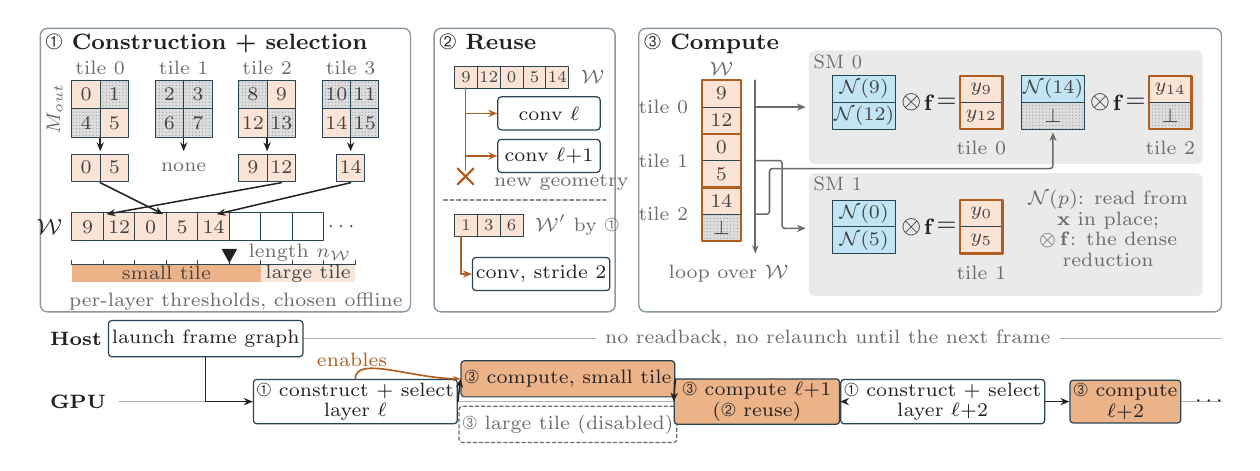
\begin{tikzpicture}[x=1mm, y=1mm]
  \def\isact#1{\pgfmathparse{or(or(or(or(#1==0,#1==5),#1==9),#1==12),#1==14)}}
  % \slot{x}{y}{w}{h}{label or empty}{fill style}
  \newcommand{\slot}[6]{\path[#6] (#1, #2) rectangle ++(#3, -#4);
    \draw[rule, line width=0.35pt] (#1, #2) rectangle ++(#3, -#4);
    \node[idx] at (#1+#3/2, #2-#4/2) {#5};}
  % \mtile{x}{y}{first index}: a 2x2 mask tile (active orange, inactive dotted)
  \newcommand{\mtile}[3]{%
    \foreach \k/\o in {0/0, 1/1, 2/4, 3/5} {
      \pgfmathtruncatemacro\i{#3+\o}\pgfmathtruncatemacro\r{\k/2}\pgfmathtruncatemacro\q{mod(\k,2)}
      \isact{\i}
      \ifnum\pgfmathresult=1 \fill[actfill] (#1+\q*3.6, #2-\r*3.6) rectangle ++(3.6, -3.6);
      \else \path[waste] (#1+\q*3.6, #2-\r*3.6) rectangle ++(3.6, -3.6); \fi
      \node[idx] at (#1+\q*3.6+1.8, #2-\r*3.6-1.8) {\i};}
    \draw[rule, line width=0.35pt] (#1, #2) rectangle ++(7.2, -7.2) (#1+3.6, #2) -- ++(0, -7.2) (#1, #2-3.6) -- ++(7.2, 0);}

  %% ---------------------------------------------------------------- (1) construction + selection
  \draw[box] (0, 0) rectangle (47, -36);
  \node[boxtitle] at (0, 0) {\num{1} Construction + selection};
  \node[note, rotate=90] at (1.8, -10.2) {$M_{out}$};
  \foreach \t/\f in {0/0, 1/2, 2/8, 3/10} {
    \mtile{4+\t*10.6}{-6.6}{\f}
    \node[note] at (4+\t*10.6+3.6, -5.0) {tile \t};
    \draw[flow] (4+\t*10.6+3.6, -14.0) -- ++(0, -1.6);}
  % segments (tile-local, in dense order inside each tile)
  \slot{4.0}{-16.0}{3.6}{3.4}{0}{fill=actfill}\slot{7.6}{-16.0}{3.6}{3.4}{5}{fill=actfill}
  \node[note] at (4+10.6+3.6, -17.7) {none};
  \slot{25.2}{-16.0}{3.6}{3.4}{9}{fill=actfill}\slot{28.8}{-16.0}{3.6}{3.4}{12}{fill=actfill}
  \slot{37.6}{-16.0}{3.6}{3.4}{14}{fill=actfill}
  % worklist W in arrival order
  \def\wy{-23.4}
  \foreach \k/\p in {0/9, 1/12, 2/0, 3/5, 4/14} \slot{4+\k*4.0}{\wy}{4.0}{3.6}{\p}{fill=actfill};
  \foreach \k in {5,6,7} \slot{4+\k*4.0}{\wy}{4.0}{3.6}{}{fill=white};
  \node[idx] at (4+8*4.0+2.2, \wy-1.8) {$\cdots$};
  \node[anchor=east] at (4.0, \wy-1.8) {$\mathcal{W}$};
  \draw[flow] (30.6, -19.6) -- (8.4, \wy-0.2);
  \draw[flow] (7.6, -19.6) -- (15.6, \wy-0.2);
  \draw[flow] (39.4, -19.6) -- (22.4, \wy-0.2);
  % length ruler with the layer's thresholds; the pointer is this frame's n_W
  \def\ry{-30.0}
  \fill[selfill] (4, \ry) rectangle (4+6*4.0, \ry-2.2);
  \fill[altfill] (4+6*4.0, \ry) rectangle (4+9*4.0, \ry-2.2);
  \node[idx] at (4+3*4.0, \ry-1.1) {small tile};
  \node[idx] at (4+7.5*4.0, \ry-1.1) {large tile};
  \foreach \k in {0,...,9} \draw[rule, line width=0.3pt] (4+\k*4.0, \ry) -- ++(0, 0.5);
  \draw[rule, line width=0.35pt] (4, \ry) -- (4+9*4.0, \ry);
  \fill[ink] (4+5*4.0, \ry+0.2) -- ++(-1.0, 1.8) -- ++(2.0, 0) -- cycle;
  \node[note, anchor=west] at (4+5*4.0+1.2, \ry+1.5) {length $n_\mathcal{W}$};
  \node[note, anchor=north west] at (2.4, \ry-2.4) {per-layer thresholds, chosen offline};

  %% ---------------------------------------------------------------- (2) reuse
  \draw[box] (50, 0) rectangle (73, -36);
  \node[boxtitle] at (50, 0) {\num{2} Reuse};
  \foreach \k/\p in {0/9, 1/12, 2/0, 3/5, 4/14} \slot{52.6+\k*2.9}{-4.8}{2.9}{2.8}{\scalebox{0.85}{\p}}{fill=actfill};
  \node[note, anchor=west] at (67.4, -6.2) {$\mathcal{W}$};
  \node[node box, minimum width=13mm, minimum height=4.2mm] (l0) at (64.6, -10.8) {conv $\ell$};
  \node[node box, minimum width=13mm, minimum height=4.2mm] (l1) at (64.6, -16.2) {conv $\ell{+}1$};
  \draw[flow, draw=wiseconv!80!black] (54.0, -7.6) |- (l0.west);
  \draw[flow, draw=wiseconv!80!black] (54.0, -7.6) |- (l1.west);
  % the chain breaks where the geometry changes
  \draw[wiseconv!80!black, line width=0.55pt] (54.0, -16.2) -- (54.0, -18.0);
  \draw[wiseconv!80!black, line width=0.8pt] (53.0, -17.8) -- ++(2, -2) (55.0, -17.8) -- ++(-2, -2);
  \node[note, anchor=west] at (56.4, -19.6) {new geometry};
  \draw[rule!60, line width=0.5pt, dash pattern=on 1.4pt off 1pt] (51.2, -21.8) -- (71.8, -21.8);
  \foreach \k/\p in {0/1, 1/3, 2/6} \slot{52.6+\k*2.9}{-23.6}{2.9}{2.8}{\scalebox{0.85}{\p}}{fill=actfill};
  \node[note, anchor=west] at (61.6, -25.0) {$\mathcal{W}'$ by \num{1}};
  \node[node box, minimum width=15mm, minimum height=4.2mm] (l2) at (63.6, -31.2) {conv, stride 2};
  \draw[flow, draw=wiseconv!80!black] (53.4, -26.4) |- (l2.west);

  %% ---------------------------------------------------------------- (3) compute
  \draw[box] (76, 0) rectangle (150, -36);
  \node[boxtitle] at (76, 0) {\num{3} Compute};
  \def\wx{84.0}\def\wh{3.4}\def\wt{-6.6}
  \foreach \k/\p in {0/9, 1/12, 2/0, 3/5, 4/14} \slot{\wx}{\wt-\k*\wh}{5.0}{\wh}{\p}{fill=actfill};
  \slot{\wx}{\wt-5*\wh}{5.0}{\wh}{$\bot$}{waste}
  \node[note] at (\wx+2.5, \wt+1.5) {$\mathcal{W}$};
  \foreach \t in {0,1,2} {
    \draw[wiseconv!80!black, line width=0.8pt] (\wx, \wt-2*\t*\wh) rectangle ++(5.0, -2*\wh);
    \node[note, anchor=east] at (\wx-0.5, \wt-2*\t*\wh-\wh) {tile \t};}
  % loop over W, handing each tile to the next free SM
  \draw[-{Stealth[length=3pt]}, line width=0.7pt, draw=muted] (\wx+6.8, \wt) -- (\wx+6.8, \wt-6*\wh-1.6);
  \node[note, anchor=north] at (\wx+3.4, \wt-6*\wh-1.8) {loop over $\mathcal{W}$};
  \draw[flow, draw=muted] (\wx+6.8, \wt-\wh) -- (97.2, \wt-\wh);
  \draw[flow, draw=muted, rounded corners=1pt] (\wx+6.8, \wt-3*\wh) -- (\wx+10.2, \wt-3*\wh) -- (\wx+10.2, -25.4) -- (97.2, -25.4);
  % persistent SMs, computing as in fig:tile-skip
  \fill[smfill, rounded corners=2pt] (97.6, -2.8) rectangle (147.6, -17.2);
  \fill[smfill, rounded corners=2pt] (97.6, -18.4) rectangle (147.6, -34.0);
  \node[smlabel] at (97.6, -2.8) {SM 0};
  \node[smlabel] at (97.6, -18.4) {SM 1};
  % tile 2 goes back to SM 0 once it frees up (drawn over the SM fill)
  \draw[flow, draw=muted, rounded corners=1pt] (\wx+6.8, \wt-5*\wh) -- (\wx+8.6, \wt-5*\wh) -- (\wx+8.6, -17.8) -- (128.6, -17.8) -- (128.6, -13.2);
  % \issue{x}{y}{p}{q}{tile}: [N(p); N(q)] (o) f = [y_p; y_q]  (q = \nil: padding)
  \def\aw{8.0}\def\ah{3.4}\def\bw{5.4}
  \newcommand{\issue}[5]{%
    \slot{#1}{#2}{\aw}{\ah}{$\mathcal{N}(#3)$}{fill=infill}
    \ifx#4\nil \slot{#1}{#2-\ah}{\aw}{\ah}{$\bot$}{waste}\else \slot{#1}{#2-\ah}{\aw}{\ah}{$\mathcal{N}(#4)$}{fill=infill}\fi
    \node[op] at (#1+\aw+2.0, #2-\ah) {$\otimes$};
    \node at (#1+\aw+4.3, #2-\ah) {$\mathbf{f}$};
    \node[op] at (#1+\aw+6.5, #2-\ah) {$=$};
    \slot{#1+\aw+8.2}{#2}{\bw}{\ah}{$y_{#3}$}{fill=actfill}
    \ifx#4\nil \slot{#1+\aw+8.2}{#2-\ah}{\bw}{\ah}{$\bot$}{waste}\else \slot{#1+\aw+8.2}{#2-\ah}{\bw}{\ah}{$y_{#4}$}{fill=actfill}\fi
    \draw[wiseconv!80!black, line width=0.8pt] (#1+\aw+8.2, #2) rectangle ++(\bw, -2*\ah);
    \node[note, anchor=north] at (#1+\aw+8.2+\bw/2, #2-2*\ah-0.3) {tile #5};}
  \def\nil{nil}
  \issue{100.6}{-6.0}{9}{12}{0}
  \issue{124.6}{-6.0}{14}{\nil}{2}
  \issue{100.6}{-21.8}{0}{5}{1}
  \node[note, align=center] at (135.6, -25.4) {$\mathcal{N}(p)$: read from\\$\mathbf{x}$ in place;\\$\otimes\,\mathbf{f}$: the dense\\reduction};

  %% ---------------------------------------------------------------- per-frame CUDA graph
  \def\hy{-39.4}\def\gy{-47.4}
  \tikzset{node box/.append style={minimum height=4.6mm}}
  \node[anchor=west, font=\fontsize{7.4}{8}\selectfont\bfseries] at (0, \hy) {Host};
  \node[anchor=west, font=\fontsize{7.4}{8}\selectfont\bfseries] at (0, \gy) {GPU};
  \draw[rule!40, line width=0.4pt] (10, \hy) -- (150, \hy) (10, \gy) -- (150, \gy);
  \node[node box, fill=white] (launch) at (21, \hy) {launch frame graph};
  \node[note, fill=white] at (100, \hy) {no readback, no relaunch until the next frame};
  \node[node box, fill=white, minimum width=22mm] (c1) at (40, \gy) {\num{1} construct + select\\layer $\ell$};
  \node[node box, fill=selfill, minimum width=17mm] (s1) at (67, \gy+2.9) {\num{3} compute, small tile};
  \node[node box, fill=white, draw=muted, dash pattern=on 1.2pt off 1pt, text=muted, minimum width=17mm] (l1) at (67, \gy-2.9) {\num{3} large tile (disabled)};
  \node[node box, fill=selfill, minimum width=21mm] (s2) at (91.0, \gy) {\num{3} compute $\ell{+}1$\\(\num{2} reuse)};
  \node[node box, fill=white, minimum width=22mm] (c3) at (114.6, \gy) {\num{1} construct + select\\layer $\ell{+}2$};
  \node[node box, fill=selfill, minimum width=14mm] (s3) at (137.8, \gy) {\num{3} compute\\$\ell{+}2$};
  \node at (148.4, \gy) {$\cdots$};
  \draw[flow] (launch.south) |- (c1.west);
  \draw[flow] (c1.east) -- (s1.west);
  \draw[wiseconv!80!black, line width=0.6pt, -{Stealth[length=2.6pt]}] (c1.north) .. controls +(0, 3.0) and +(-6, 0) .. (s1.west)
    node[pos=0.5, above left, note, text=wiseconv!80!black, inner sep=0.8pt] {enables};
  \draw[flow] (s1.east) -- (s2.west);
  \draw[flow] (s2.east) -- (c3.west);
  \draw[flow] (c3.east) -- (s3.west);
\end{tikzpicture}
\end{document}
